\documentclass[11pt, oneside, a4paper]{report}  

% Input and math
\usepackage[utf8]{inputenc}
\usepackage{amsmath,amssymb,amsfonts}
\usepackage{amsthm}

% Hyperlinks
\usepackage{hyperref}

% Colors
\usepackage{color}
\definecolor{dkgreen}{rgb}{0,0.6,0}
\definecolor{gray}{rgb}{0.5,0.5,0.5}


% Source code listings (see below begindoc), graphics
\usepackage{listings}
\usepackage{graphicx}
\usepackage{subfig}

\begin{document}

% For source code listings
\lstset{language=Matlab,
   keywords={break,case,catch,continue,else,elseif,end,for,function,
      global,if,otherwise,persistent,return,switch,try,while},
   basicstyle=\ttfamily,
   keywordstyle=\color{blue},
   commentstyle=\color{red},
   stringstyle=\color{dkgreen},
   numbers=left,
   numberstyle=\tiny\color{gray},
   stepnumber=1,
   numbersep=10pt,
   backgroundcolor=\color{white},
   tabsize=4,
   showspaces=false,
   showstringspaces=false}

\title{Blind Source Separation}
\author{}
\date{}    % type date between braces
\maketitle

\begin{abstract}

\end{abstract}

\tableofcontents

\chapter{Introduction}

Blabla... gpp

\section{Formal Problem Statement}

We now provide a notation leading to a mathematical statement of the blind source separation (BSS) problem. We let $\boldsymbol{S}(t)\in \mathbf{R}^n$ for $t>0, n>0$ denote the signals generated by $n$ sources. Similarly, let $\boldsymbol{X}(t)\in \mathbf{R}^m$ for $t>0, n>0$ the observed sensor readings resulting from the emitted signals. A \emph{mixing model} $f(\boldsymbol{S},t)$ defines the relationship between source and observed signal:

\begin{equation}\label{mixing_model}
  \boldsymbol{X} = f(\boldsymbol{S},t)
\end{equation}

As only the observed value $\boldsymbol{X}$ is known, we need to determine the inverse $f^{-1}(\boldsymbol{S},t)$, that is, the \emph{unmixing model}.

\subsection{Single Sensor Blind Source Separation}

A particular instance of the BSS problem, is the single sensor blind source separation (SSBSS) problem, to which we will devote particular attention. In the SSMSS problem, we have one or more source signals, but the observed signal $\boldsymbol{X}(t)$ is a scalar. This introduces problems as this instance does not lend itself to solutions by means of the ``standard'' methods we consider in the standard BSS problem. Chapter \ref{ssbss_chap} is devoted to the SSBSS problem.

\subsection{A Linear Mixing Model}

The simplest mixing model is a noiseless, stationary linear mixing model. The stationarity assumption means that the mixing model does not change as a function of time, so the $t$ argument in Equation \ref{mixing_model} can be omitted. With $T$ measurements, $N$ sources, and $M$ sensors, this model can be defined as:


\begin{equation}\label{linear_mixing_model}
  X = AS
\end{equation}

With $\boldsymbol{}X \in \mathbf{R}^{N\times T}$, $\boldsymbol{A} \in \mathbf{R}^{N\times M}$
and $\boldsymbol{S} \in \mathbf{R}^{M\times T}$. The problem of determining the
unmixing model now consists of computing the inverse $\boldsymbol{W} = \boldsymbol{A}^{-1}$, so
that the original signal:

\begin{equation}\label{linear_unmixing_model}
\boldsymbol{S} = \boldsymbol{W}\boldsymbol{X}
\end{equation}

can be recovered. This is to say that the estimate of the original
signal $j$ at time $t$ is computed as the $j$th row of $\boldsymbol{W}$ times the
$t$th column of $X$.

From Equation \ref{linear_mixing_model}, we can see that the blind source separation problem, even in the simplest case, is ill-poised, as we are trying to determine $M\times T + N\times M$ parameters (both $A$ and $S$) given only $N\times T$ ($\boldsymbol{X}$). This implies that we need to impose some kind of assumptions on the nature of the data. These assumptions, often called the \emph{generative model}, state something about the nature of the signals and how they are mixed. As will be made apparent later, which assumptions are made, gives rise to different solution approaches. For the purpose of this study, we will be quite restrictive in what assumptions we are willing make, hence the term \emph{blind} source separation. The type of assumptions made are primarily related to statistical properties of the sources. The textbook assumptions are uncorrelated and independendent sources, leading to the PCA and ICA solutions, respectively\footnote{Under the assumptions that the number of observations are greater than or equal to the number of sources.}.

\section{Overview}

In the next chapters we will be looking at a few different algorithms for solving various instances of the BSS problem. Each algorithm has its own merits depending to a large extent on the assumptions we make about the data. An overview of these follow in the Table \ref{overviewTable}.

\begin{center}
  \begin{table}[h!]
    \begin{tabular}{ | l | l | l | p{5cm} |}
      \hline
      \textbf{Data characteristic} & \textbf{Method} & \textbf{Description} \\ \hline
      Uncorrelated sources. & PCA & Blablabla \\ 
      Independent, non-gaussian sources. & ICA & blabla \\
      Fewer sources than observations. & HMM & blabla \\
      \hline
    \end{tabular}
    \caption{Overview over the different approaches to blind source separation covered in this report.}
    \label{overviewTable}
  \end{table}
\end{center}

\chapter{Principal Component Analysis}

Principal component analysis \cite{pearson1901} (PCA) is a eigenvector-based,
non-probabilistic technique that uses orthogonal projection to
represent data in a lower dimensional subspace spanned by the $k$
first eigenvectors of the covariance matrix. The eigenvectors form an
orthogonal basis for the data such that a projection onto the
eigenvectors will decorrelate the data. In the next section we will
derive this result by maximizing the variance of an axis of projection.

PCA is useful in several applications, hereunder visualization and
detection of so-called \emph{latent variables}. The principal
components (PCs) are the basis of the subspace onto which the data is
projected, and are such that the variance explained by each component
is maximized; that is, the first PC explains a higher proportion of
variance than the second PC and so forth. We can therefore, by
retaining only the first few components acheive a representation of
the data containing the most of the variance exhibited by the
assumption that the PCs accounting for the smallest portion of
variance are noise.


The next section presents PCA from two different but equivalent
perspectives; first solving for the direction of maximal variation
using the method of Lagrange multipliers, and subsequently by singular
value decomposition which. The latter is the more computationally
efficient, and the rationale for this approach is easy to see once the
first perspective is known. We then proceed to looking at how PCA can
be applied to the blind source problem, before we finally look at a
non-linear extension of PCA.


\section{Formal Statement}

Let $\boldsymbol{x}_i \in \mathbf{R}^n$ denote the $i$'th observation of a dataset
of $m$ observations. We now want to project our data onto a vector $\boldsymbol{u}$
in $\mathbf{R}^n$ so as to maximize the variance of the resulting
projection $\sum_{i=1}^m \boldsymbol{x}_i^T \boldsymbol{u}$ subject to the constraint
$|\boldsymbol{u}|=1$. Under the assumption that $\boldsymbol{X}$ is standardized to zero mean
and unit variance, the Lagrangian is then given by Equation \ref{pca_lagrangian}:

  \begin{equation}
    \label{pca_lagrangian}
    \begin{array}{lcl}
      \mathcal{L}(u,\lambda) & = & \frac{1}{m} \sum_{i=1}^m (\boldsymbol{x}_i^T \boldsymbol{u})^2 - \lambda (\boldsymbol{u}^T \boldsymbol{u} -1) \\
      \\& = & \frac{1}{m} \sum_{i=1}^m (\boldsymbol{u}^T \boldsymbol{x}_i)^T(\boldsymbol{x}_i^T \boldsymbol{u}) - \lambda (\boldsymbol{u}^T \boldsymbol{u} -1) \\
      \\& = & \frac{1}{m} \sum_{i=1}^m \boldsymbol{u}^T(\boldsymbol{x}_i \boldsymbol{x}_i^T)u - \lambda (\boldsymbol{u}^T \boldsymbol{u} -1) \\
      \\& = & \frac{1}{m}  u^T\sum_{i=1}^m(\boldsymbol{x}_i \boldsymbol{x}_i^T)\boldsymbol{u} - \lambda (\boldsymbol{u}^T \boldsymbol{u} -1) \\
      \\& = & \frac{1}{m} \boldsymbol{u}^T \boldsymbol{\Sigma} \boldsymbol{u} - \lambda (\boldsymbol{u}^T \boldsymbol{u} -1) \\
    \end{array}
  \end{equation}

Here, $\boldsymbol{\Sigma} = \sum_{i = 1}^m \boldsymbol{x}_i \boldsymbol{x}_i^T$ is the covariance matrix. Setting the gradient of \ref{pca_lagrangian} equal to zero yields Equation \ref{pca_gradient}:

\begin{equation}
  \label{pca_gradient}
  \nabla_u \mathcal{L}(\boldsymbol{u}, \lambda) = \boldsymbol{\Sigma} \boldsymbol{u} - \lambda \boldsymbol{u} = 0
\end{equation}

Equation \ref{pca_gradient} shows that the direction of maximum variance $u$, which we will refer to as the first principal component, is the first eigenvector of the covariance matrix of the dataset. By similar means it can be shown that the second eigenvector points in the direction of largest variance \emph{orthogonal} to the first eigenvector and so forth. Finally it is worth noting that the portion of the total variance explained by a principal component is proportional to its associated eigenvalue.

\subsection{Singular Value Decomposition}

For a high dimensional dataset (e.g. $n = 10,000$), which is
frequently the case working with for instance image or video data, the covariance matrix will have $10,000\times 10,000 = 100,000,000$ entries, which is computationally untractable. Hence, PCA is usually implemented in terms of \emph{singular value decomposition} (SVD). For an $m\times n$ matrix $\boldsymbol{X}$, the SVD is a factorization such that:

\begin{equation}
  X = US V^{T}
\end{equation}

Here, $U \in \mathbf{R}^{m\times m}$, $S \in \mathbf{R}^{m\times n}$,
and $U \in \mathbf{R}^{n\times n}$. The SVD relates to the eigenvalue
problem (Equation \ref{pca_gradient}) as follows:

\begin{itemize}
\item The columns of $U$ form the projections of $X$ onto the
  eigenvectors $V$.
  \item The entries $s_{ii}$ on the leading diagonal of $S$ are the
    eigenvalues of $\Sigma = X^TX$.
  \item The top $k$ columns of $V$ are the top $k$ eigenvectors of
    $\Sigma = X^T X$
\end{itemize}

In \textsc{Matlab}, we can perform SVD by a single line of code
(subsequent to standardizing the data to zero mean and unit variance):

\begin{figure}[!htpb]
  \begin{lstlisting}[frame=single]
   [U,S,V] = svd(X' * X);
  \end{lstlisting}
  \caption{\textsc{Matlab} code for SVD.}
  \label{svd_code}
\end{figure}

We will not go into the derivation of this result as SCD is covered
in most textbooks on linear algebra or basic numerical
mathematics. Rather, we will proceed to show how PCA can be applied to
BSS, and what assumptions it requires us to make about the data.



\section{PCA Application to Blind Source Separation}\label{pca_bss}
% TODO: update graphs to newest version

The top graph of Figure \ref{pca_time_series} shows two periodic signals $s_1$ and $s_2$ contaminated by an additive Gaussian white noise with standard deviation $\sigma = .2$.

\begin{equation}
      \begin{array}{lll}
        s_1 = & \sin(\pi x) & 0<x<5\\
        s_2 = & \cos(7 \pi x) & 0<5<x\\
    \end{array}
\end{equation}

The signals are subsequently mixed, as shown in the middle part of Figure \ref{pca_time_series} by the matrix:

\begin{equation}
  A = \begin{bmatrix} \cos \alpha & -\sin \alpha \\ \sin \alpha & \cos \alpha \end{bmatrix}
\end{equation}

where $\alpha = \pi/4$. Here the mixing matrix $A$ corresponds to a rotation operator that will rotate the data by $\alpha$ radians in counterclockwise direction. 

The lower part of Figure \ref{pca_time_series} shows the recovered signal\footnote{The estimated unmixing matrix here is $\hat{W} = \hat{A}^{-1} = \begin{bmatrix} .7071 & .7071 \\ -.7071 & .7071 \end{bmatrix}$ which is, as expected, the inverse of $A$ for the value of $\alpha$ above.}.

\begin{itemize}
  \item Example where it works - why
  \item Example where it fails - why
\end{itemize}



\begin{figure}
  \centering
  \hrule
  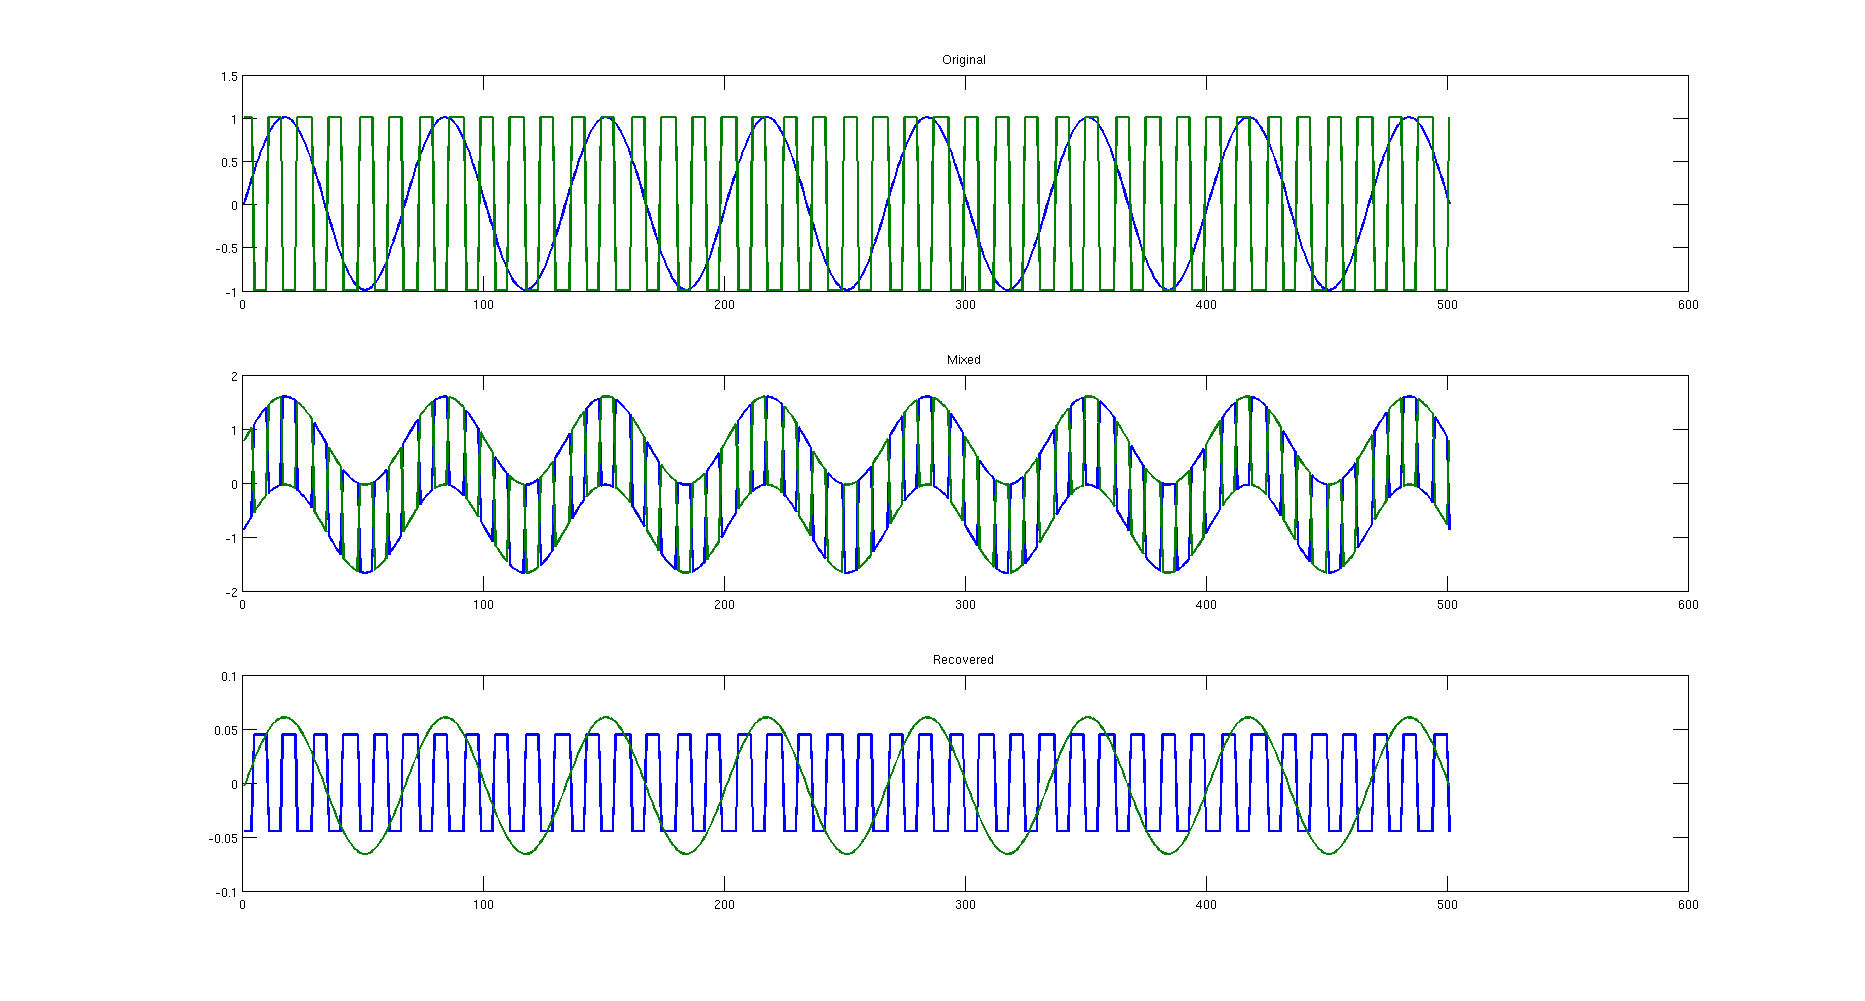
\includegraphics[width = .9\textwidth]{Figures/pca_signal_time_series}
  \hrule
  \caption{PCA Source Separation.}
  \label{pca_time_series}
\end{figure}

\begin{figure}
  \centering
  \hrule
  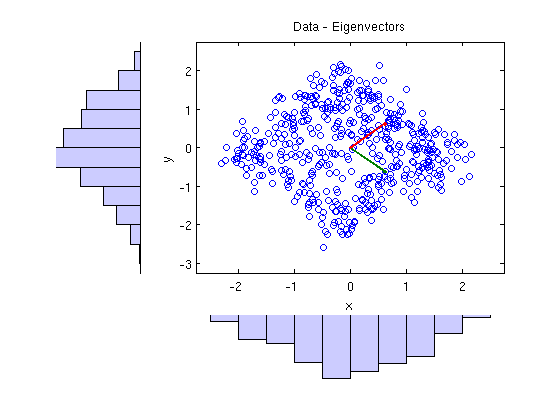
\includegraphics[width = .9\textwidth]{Figures/pca_data_eigs}
  \hrule
  \caption{Standardized data points vs eigenvectors.}
\end{figure}

\begin{figure}
  \centering
  \hrule
  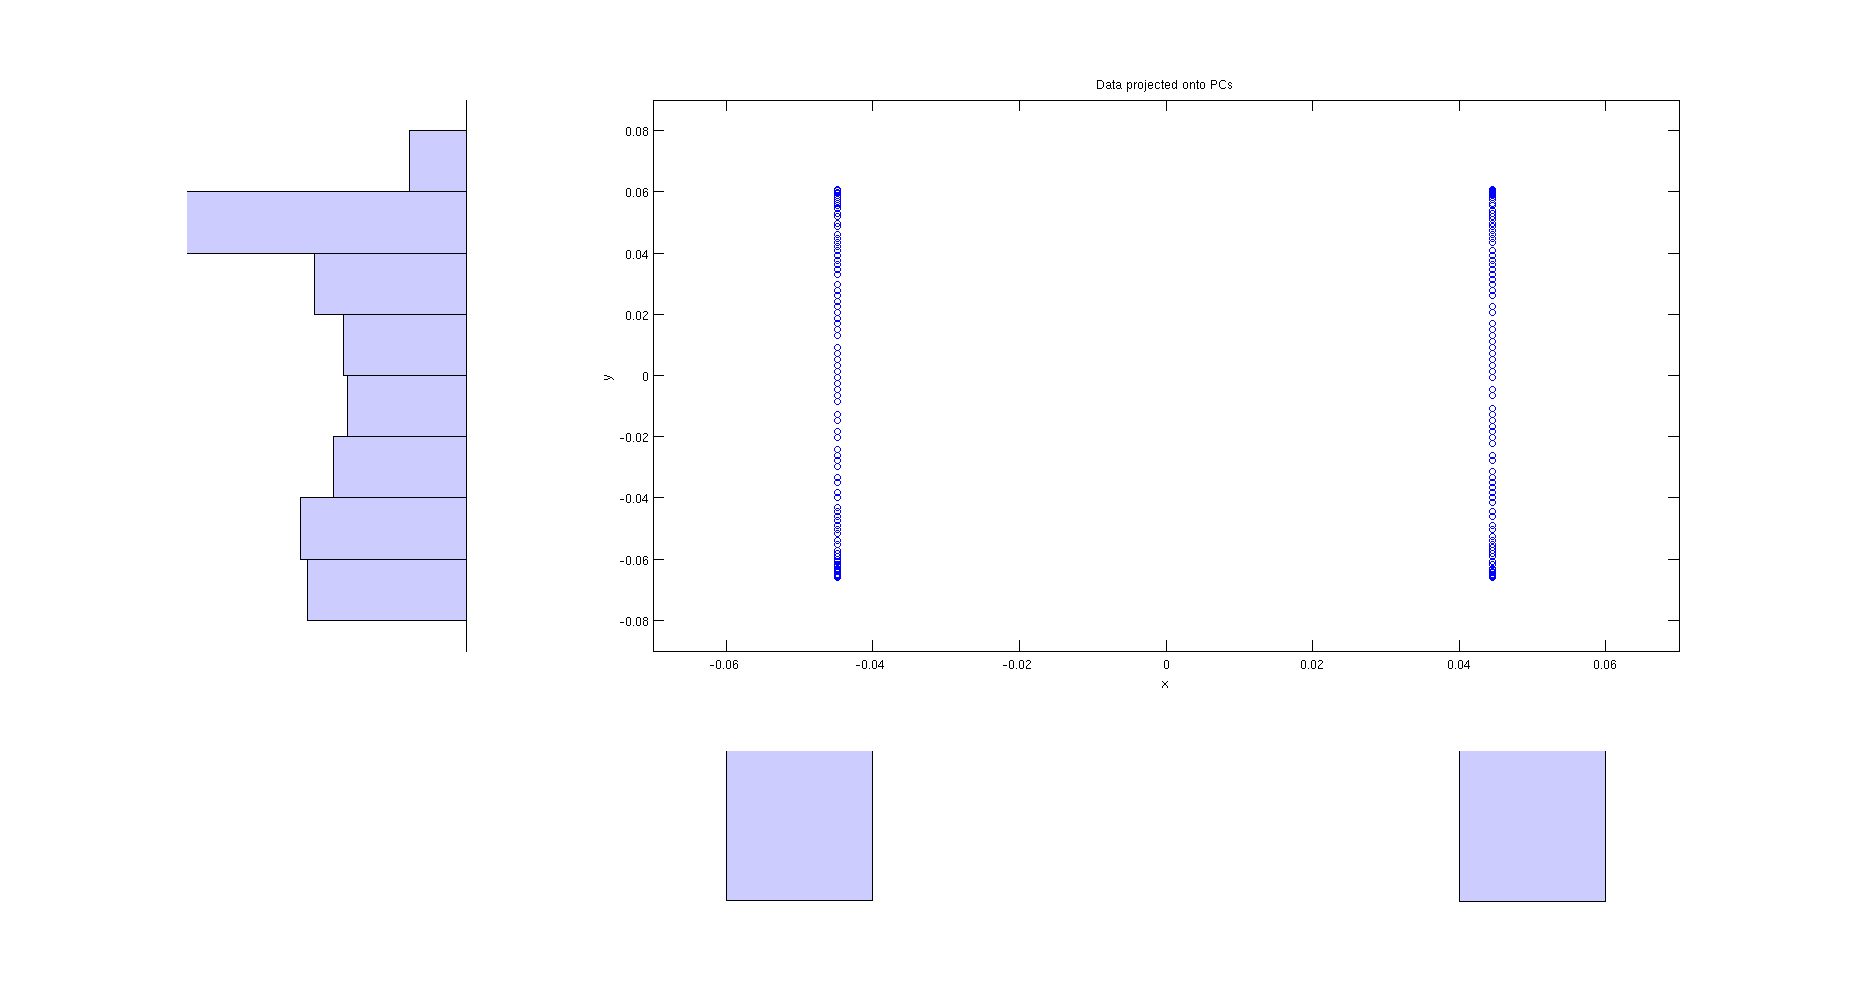
\includegraphics[width = .9\textwidth]{Figures/pca_eig_projection}
  \hrule
  \caption{Standardized data projected onto eigenvectors.}
\end{figure}

\chapter{Independent Component Analysis}

PCA finds the basis of a subspace in which the variance is
maximized in the direction of the basis vectors and the covariance
between the data is zero. ICA seeks to find basis
vectors that are statistically independent, which is a stronger
property than simply being uncorrelated as independence implies
uncorrelatedness, while the opposite is not true. ICA in contrast to PCA does not have analytic solutions in the general case, 
so a numerical optimization method is usually applied in computing the ICA transform.

\section{Limitations of the ICA Model}\label{ICA_restrictions}

\begin{itemize}
  \item Non-Gaussian..
  \item Ordering of signals..
  \item ``Sign reversal'' (rotational invariance??)..
  \item Blabla..
\end{itemize}


\section{ICA in the Linear Mixing Model}

\subsection{Equivalent Specifications of ICA}

ICA can be derived by several different approaches:
\begin{itemize}
  \item Maximum likelihood
  \item Kurtosis maximization
  \item Maximum differential entropy
  \item Blabla..
\end{itemize}



\subsection{Maximum Likelihood Derivation}\label{ml_ica}

Let $p_s(s_i)$ be the probability density function for source $i$, then, assuming the sources are independent the joint distribution of all the $n$ sources is given by the product of the marginals:

\begin{equation}
  p(s) = \Pi_{i=1}^n p_s(s_i)
\end{equation}

We now substitute in the unmixing model (Equation \ref{linear_unmixing_model}) and obtain:

\begin{equation}
  p(s) = \Pi_{i=1}^n p_s(WX) \cdot |W|
\end{equation}

The unmixing matrix is the target parameter of our maximum likelihood approach. That is, we seek set the coefficients of the unmixing matrix so as to maximize the likelihood of observing the actual data. If our dataset consists of $T$ observations $X = \{x_1,x_2,...,x_T\}$, the log-likehliood function is:

\begin{equation}
  l(W) =\log Prob(X|W)= \Sigma_{t=1}^T \log p_s(WX)+\log |W|
\end{equation}

As the ICA is incompatible with a Gaussian source distribution, common choices for specifying $P_s$ include the sigmoid $p_s(s) = \frac{1}{1+e^{-s}}$ and hyperbolic tangent ($\tanh(s)$).

\begin{figure}[!htpb]
  \begin{lstlisting}[frame=single]
    code here...?
  \end{lstlisting}
  \caption{\textsc{Matlab} code for ML ICA by gradient descent.}
  \label{mlica_code}
\end{figure}



\subsection{Preprocessing}\label{ica_preprocessing}

Whitening transform...

STFT?

\section{BSS by ICA}\label{BSS_ICA}


\begin{figure}
  \centering
  \hrule
  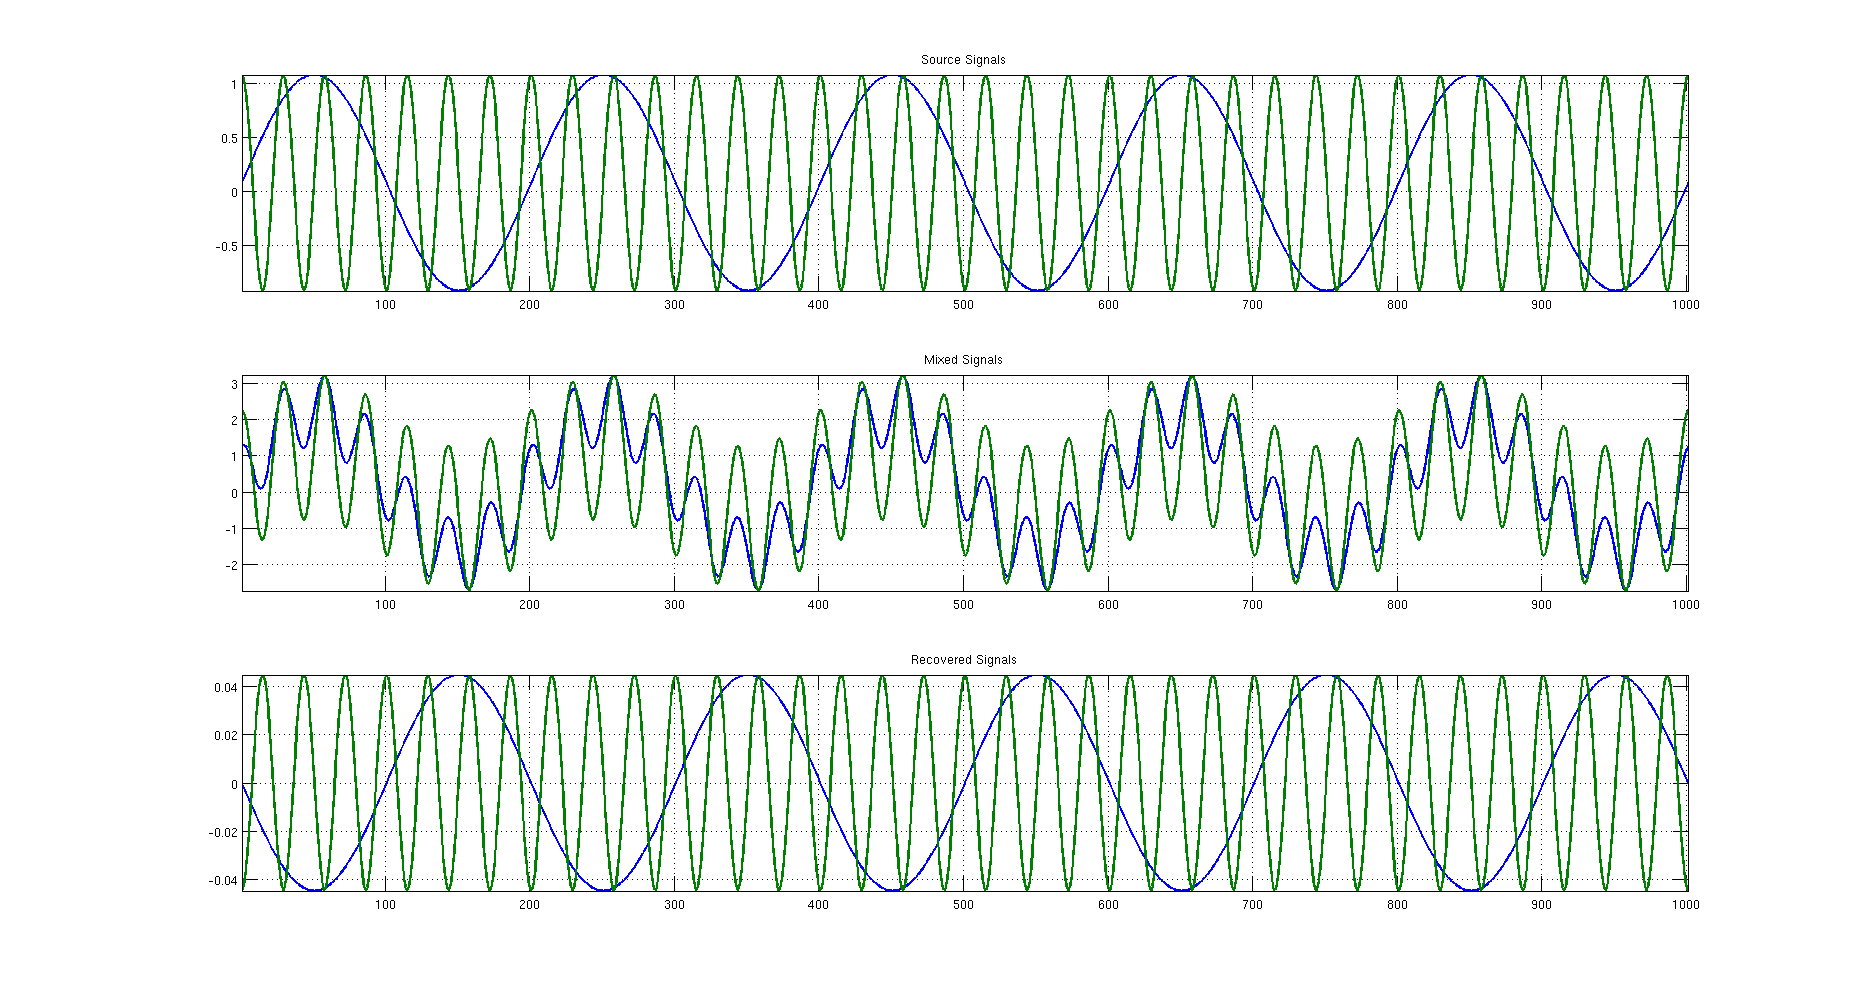
\includegraphics[width = .9\textwidth]{Figures/ica_simple}
  \hrule
  \caption{ICA on a $2\times 2$ BSS problem. Note the ``sign reversal'' for the blue sine wave (cf. Section \ref{ICA_restrictions}).}
\end{figure}

\begin{figure}
  \centering
  \hrule
  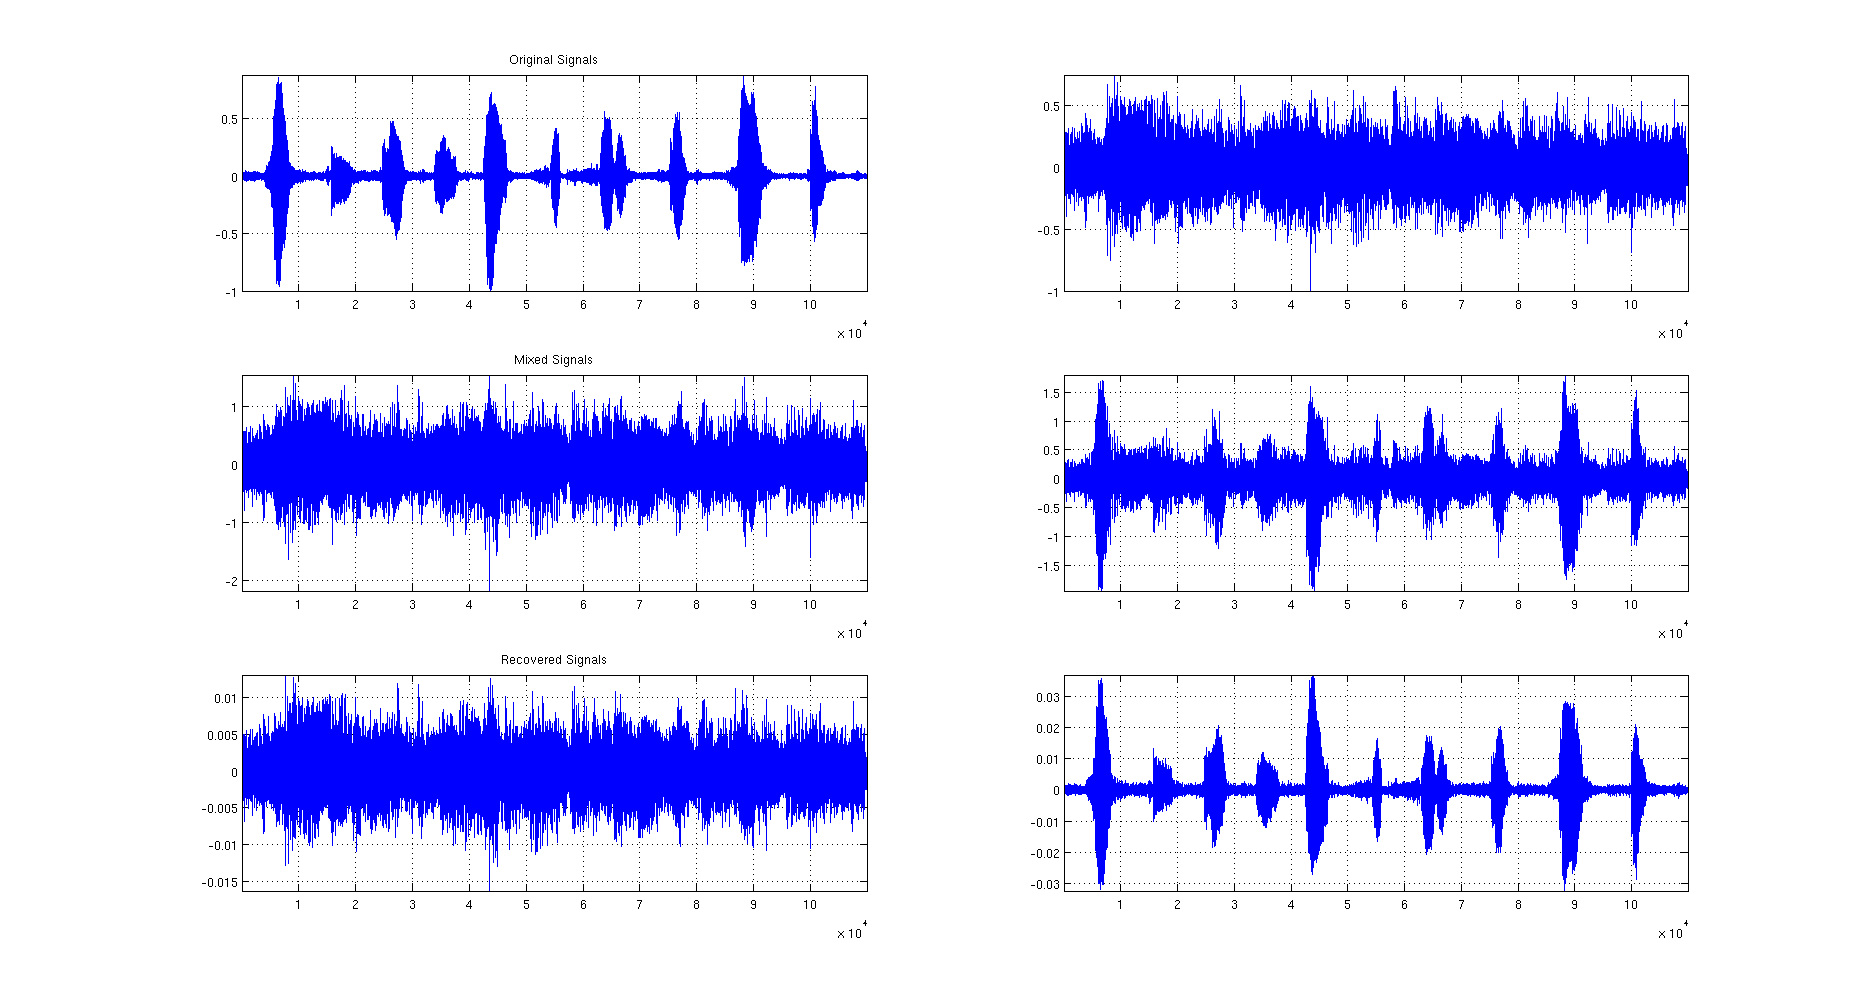
\includegraphics[width = .9\textwidth]{Figures/ica_music_speech}
  \hrule
  \caption{Separating a speech signal (top left) from background music (top right) by ICA. Here we also observe that the sign of the original speech signal is reversed in the bottom right recovered signal. }
\end{figure}




\section{Limitations and Comparison with PCA}\label{ica_conclusions}

Refer to section \ref{pca_bss} in discussion.


\chapter{Single Sensor Blind Source Separation}\label{ssbss_chap}

todo.



\section{Inference in Hidden Markov Models}




\chapter{Conclusion}

todo.


\appendix
\chapter{Some Mathematical Concepts}

In this appendix we will provide a brief background on some of the mathematical notions that are central to understanding the methods used in this report. 

\section{Linear Algebra}

% the easy stuff
In this section we will define a few important concepts that are
necessary, in particular for the PCA method.

\subsubsection{T}

\section{Statistics and Optimization}

% ML-estimation + gradient descent
A large portion of machine learning relies on statistical
methods; the methods considered in this report being no exception. And
as the learning problems having relevance in practical life are often
far too complex to describe by analytic formulae, we therefore often
need mathematical methods to find models that have the best fit to the
observed data. In this section, we therefore consider one very
important method for finding ``optimal'' parameters in a given model,
the maximum likelihood method, as well as studying approaches to
solving it, both analytically and numerically.

\subsection{Maximum Likelihood Estimation}\label{ml-estimation}

ML estimation is a method for determining the parameters of a
statistical model by setting the parameters so as to maximize the
\emph{likelihood} of observing the actual data under the given
model. Denoting $f(\boldsymbol{X}|\boldsymbol{\Theta})$ the
probability distribution of $\boldsymbol{X} = \{x_1,x_2,...,x_n\}$
with parameters $\boldsymbol{\Theta} = \{\theta_1, \theta_2, ...,
\theta_m\}$, the maximum likelihood estimate of $\Theta$ solves Equation\ref{ml-generic}

\begin{equation}
  \label{ml-generic}
  \arg \max_\Theta f(\boldsymbol{X}|\boldsymbol{\Theta})
\end{equation}

An important case is if the $x_i$ are i.i.d., where the joint density
is the product of the marginal densities. This means we can write the
likelihood function $f$ as Equation \ref{ml-iid}.

\begin{equation}  
  \label{ml-iid}
  f(\boldsymbol{X}|\boldsymbol{\Theta}) = \prod_{i = 1}^n f(x_i|\Theta)
\end{equation}

The solution to an optimzation problem is the same under any monotone transformation. Therefore it is often times useful to deal with the log-likelihood function instead of $f$ directly.


\subsection{Some Notions in Mathematical Optimization}



\subsubsection{The Lagrange Multiplier Method}



\subsubsection{Gradient Descent}




\section{Spectral Analysis}

In working with hidden markov models for blind source separation, we
rely on a redundant signal representation in the time-frequency
domain, rather than the standard representations in the time
domain. Such a representation is advantageous in comparison with a
pure spectral representation as the latter contains no information on
when different components of a signal occur in time. While many
different time-frequency representations exist, our presentation
relies on the \emph{short-term Fourier transform} (STFT).

The time-frequency representation, often called a \emph{spectrogram} produced by the STFT maps the
energies in various parts of the spectrum over the timespan of the
signal. For a low amplitude portion of the signal will have its energy
concentrated in the upper part of the spectrogram and vice versa. This
is illustrated in Figure XX.

[[[[[[[[[[ FIGURE HERE!!! ]]]]]]]]]

\subsection{Formal statement}

Equation \ref{stft} defines the discrete time STFT for the $n$th
segment (which is centered around $m$):

\begin{equation}\label{stft}
  \text{STFT}\{x[n]\}(m,\omega)= X(m,\omega) =\sum_{n = -\infty}^{\infty}
  x[n]\omega[n-m]e^{-i\omega n}
\end{equation}

Here, $\omega$ is a zero centered window function, typically uniform
or gaussian. The window determines which part of the signal $x$ is to
be included in the spectrogram near $m$. In practice, the STFT is
computed using the fast fourier transform (FFT). To better allow for
visualization of the STFT, which is a complex number, the spectrogram
is defined as the squared magnitude ofthe STFD (Equation \ref{spectrogram}).

\begin{equation}\label{spectrogram}
  \text{spectrogram}\{x[n]\}(m,\omega) = |X(m,\omega)|^2 
\end{equation}

\begin{thebibliography}{9}

\bibitem{pearson1901}{Pearson, K. (1901). "On Lines and Planes of Closest Fit to Systems of Points in Space". Philosophical Magazine 2 (6): 559–572.}


  
\end{thebibliography}

\end{document}

